%%%%%%%%%%%%%%%%%%%%%%%%%%%%%%%%%%%%%%%%%%%%%%%%%%%%%%%%%%%%

%
% Evoflock: evolved inverse design of multi-agent motion
% speculative draft paper
%
% May 29, 2025  Begin draft.
%
%%%%%%%%%%%%%%%%%%%%%%%%%%%%%%%%%%%%%%%%%%%%%%%%%%%%%%%%%%%%

\documentclass[letterpaper]{article}
\usepackage{natbib,alifeconf}

% Used for ALife, not sure I still need them.
\usepackage{calc}
\usepackage[hyphens]{xurl}
\usepackage{hyperref}
\usepackage{tabularx}

% Added 20230421 to allow SIGGRAPH-style “teaser figure'' under title.
\usepackage{authblk}
\usepackage{titlepic}
\usepackage{caption}
\usepackage{float}
\usepackage[T1]{fontenc} % ??? QQQ -- "<"

%%%%%%%%%%%%%%%%%%%%%%%%%%%%%%%%%%%%%%%%%%%%%%%%%%%%%%%%%%%%

% \graphicspath{ {images/} {images/fcd5/} }
\graphicspath{ {images/} }

%% For introducing terms which have a special meaning in this work.
\newcommand{\jargon}[1]{\textit{#1}}

%% Use like: {\runID backyard\_oak\_20230113\_2254}
\newcommand{\runID}{\footnotesize}

%% for laying out a row of 4, 6, or 9 images
\newcommand{\igfour}[1]{\includegraphics[width=0.24\linewidth]{#1}}
\newcommand{\igsix}[1]{\includegraphics[width=0.16\linewidth]{#1}}
\newcommand{\ignine}[1]{\includegraphics[width=0.104\linewidth]{#1}}

% small fixed-width font
\newcommand{\stt}[1]{{\small \texttt{#1}}}

%%%%%%%%%%%%%%%%%%%%%%%%%%%%%%%%%%%%%%%%%%%%%%%%%%%%%%%%%%%%

\begin{document}

\title{Evoflock: evolved inverse design of multi-agent motion}

\author{Craig Reynolds\authorcr
    unaffiliated researcher\authorcr 
    cwr@red3d.com}

%%%%%%%%%%%%%%%%%%%%%%%%%%%%%%%%%%%%%%%%%%%%%%%%%%%%%%%%%%%%%%%%%%%%%%%%%%%

\captionsetup{hypcap=false}

\titlepic{
\includegraphics[width=\textwidth]{images/temp_fig_1.png}
\captionof{figure}{Boids flocking in a space cluttered with obstacles. Behavioral parameters of the boids are determined by inverse design, using multi-objective evolutionary optimization.} 
\label{fig:boid_flock}}

% Remove today's date being inserted after the title/author information.
\date{}

%% Lay out the single column top matter defined above.
\maketitle

% This puts a page number at the bottom center, but too close to text.
% \pagestyle{plain}
% \pagenumbering{arabic}

%%%%%%%%%%%%%%%%%%%%%%%%%%%%%%%%%%%%%%%%%%%%%%%%%%%%%%%%%%%%

\begin{abstract}
    This paper describes an automatic method for adjusting or tuning multi-agent motion models. Simulating the motion of bird flocks, human crowds, vehicle traffic, and other multi-agent systems is a widely used computational technique. These simulations model the behavior of a group member (bird, human, or vehicle). The group behaviors (flock, crowd, traffic) emerge from interactions between group members. These models tend to have many numeric control parameters. Although each parameter is understandable in isolation, their interaction can be complex and nonlinear. It can be difficult to know how to adjust which parameters to make a desired change in the group behavior. Changing one aspect of group behavior often causes other aspects to change, leading to a long process of incremental changes. In this work, the desired group behavior is measured with an objective(/fitness/loss) function and optimized with a genetic algorithm.
\end{abstract}

\noindent{\small\textbf{Keywords:} boids, inverse design, optimization, evolutionary computation, genetic algorithm, flocks, herds, schools, crowds, traffic}

%%%%%%%%%%%%%%%%%%%%%%%%%%%%%%%%%%%%%%%%%%%%%%%%%%%%%%%%%%%%

\begin{figure*}[t]
    \centering
    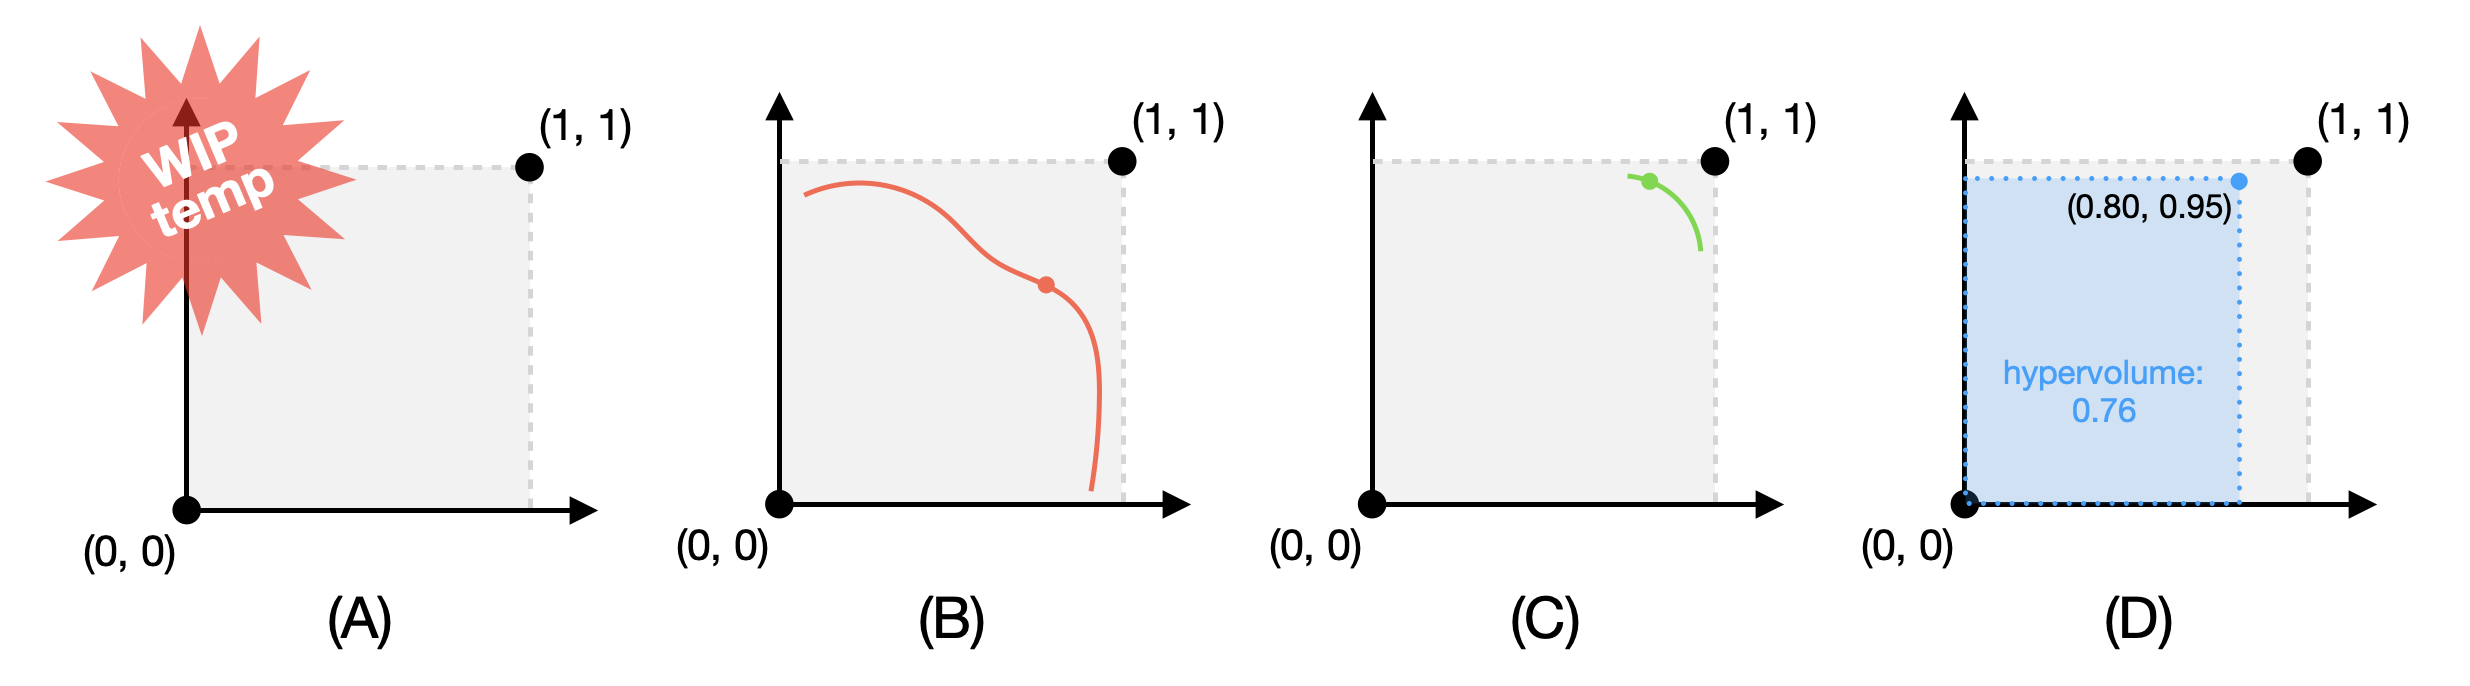
\includegraphics[width=0.9\textwidth]{images/temp_MOF_HV.png}
    \caption{(A) Normalized multi-objective fitness space. For two objectives, each with scores ranging over [0, 1], a 2D square. (B) The \textit{Pareto front} for two mutually conflicting objectives. (Like \textit{reliability} and \textit{cheapness} in the hypothetical bridge design example.) All the objectives can not be well satisfied at the same time. This is seen in the distance from (1,1) to the red curve. (C) Mostly compatible objectives, more typical of criteria for flock tuning. (D) Scalarization of a multiple-objective fitness value, using \textit{hypervolume}: the product of all objective scores. In this 2D example it is the blue rectangle's \textit{area}. [[[\textbf{TEMP}]]]}
    \label{fig:MOF_HV}
\end{figure*}

\begin{figure*}[t]
    \centering
    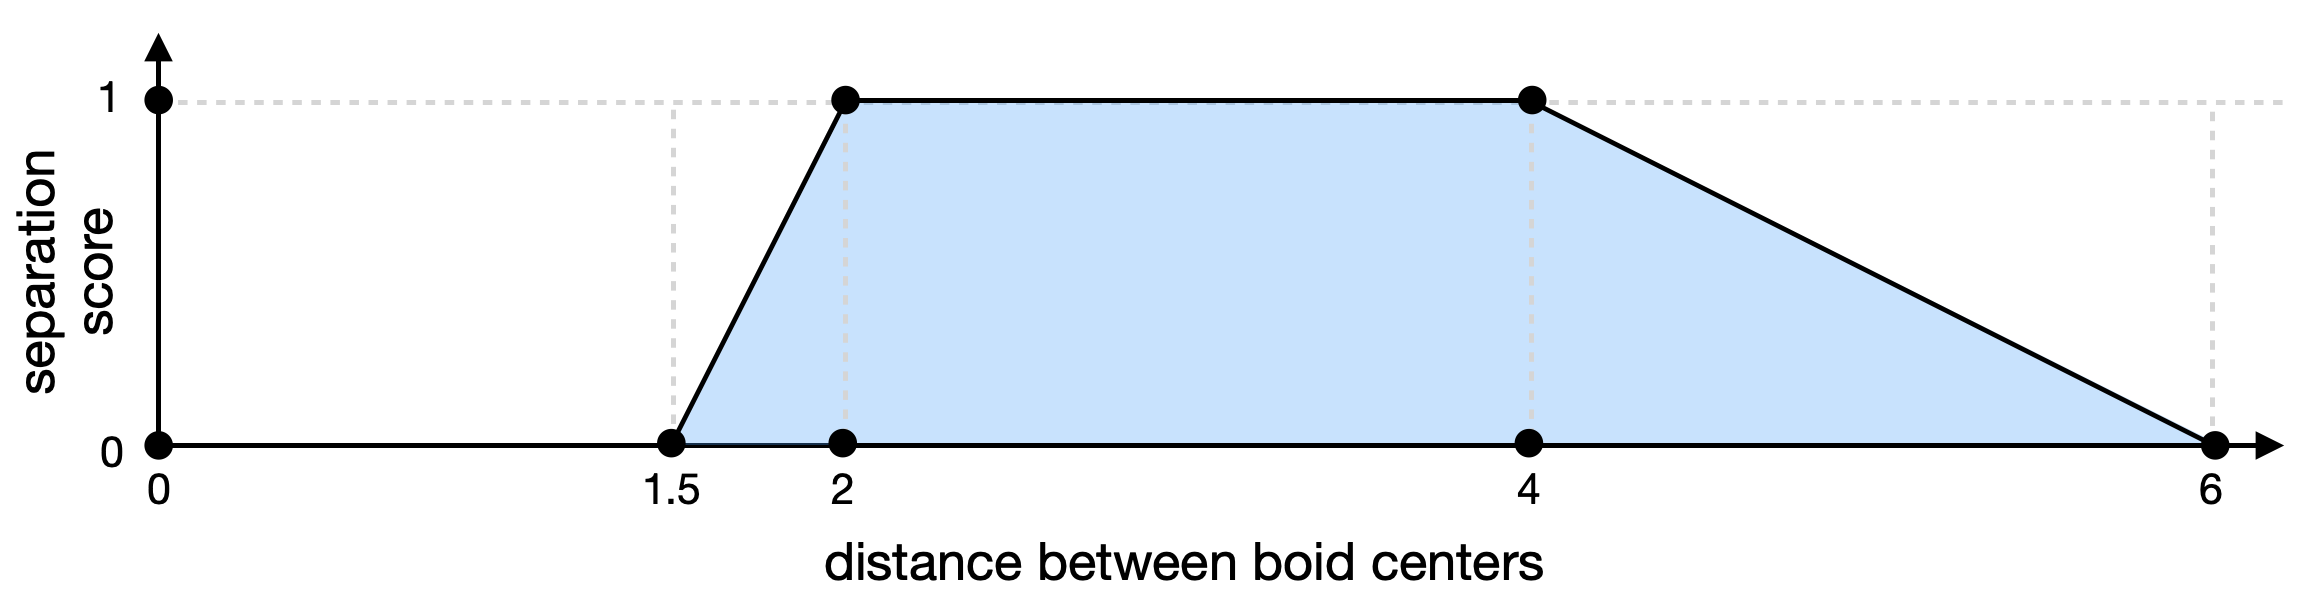
\includegraphics[width=0.9\textwidth]{images/temp_sep_score.png}
    \caption{Score for desired \textit{separation} distance to a boid's nearest neighbor. This function is highest when the centers of two boids are between 2 and 4 body diameters apart. The default boid body diameter is 1. The \textit{separation} score for an entire flock simulation is the average of this function, over all boids, on all simulation steps. [[[\textbf{TEMP}]]]}
    \label{fig:separation_score}
\end{figure*}

%%%%%%%%%%%%%%%%%%%%%%%%%%%%%%%%%%%%%%%%%%%%%%%%%%%%%%%%%%%%

\section{Introduction}
\label{sec:intro}

Simulation models of multi-agent motion are used in many fields, including: animation, games, biology, robotic swarms, and urban planning. Several early models include \textit{boids} \citep{reynolds_flocks_1987} and others (see \nameref{sec:related}). All allow creating simulations of flocks, and other group motions.  They tend to produce motion that most observers would recognize as some sort of flock. This paper will refer to bird flocks, with the assumption that other types of group motion (herds, schools, crowds, traffic) can be portrayed with suitable adjustment of the model.

This project addresses the issue of \textit{adjusting} or \textit{tuning} multi-agent motion models. For example, modifying a model of bird flocks to instead portray fish schools. Or starting from a model of flocking crows and changing it to represent a flock of sparrows. Or to take a faithful model of a birds flock in nature, and change it, say for storytelling purposes, to convey a flock of birds that are happy, or angry. Similarly, to take a generic flock model, and fit it to observations of a given species of real birds in nature.

A boids-like simulation model usually has a collection of numeric parameters that control its action. The theme of this work is to automatically determine a set of near-optimal parameters for a simulation-based multi-agent system. The flock model used for these experiments is a predefined hand-written ``black box'' model whose input is a parameter set (consisting of about about 20 numbers). A user provides a fitness(/objective/loss) function which takes a candidate parameter set, runs a simulation, and returns a score reflecting how well the behavioral goals were met. The optimization process runs (for about two hours on a laptop) and produces a high quality parameter set.

Initially, adjusting the parameters is required simply to create group motion that looks like plausible flocking. Any sort of modification to a group motion model, such as the examples mentioned above, required further adjustments to the parameters. Each such adjustment requires selecting which parameter(s) to change, whether it should increase or decrease, and by how much. Often more than one parameter needs changing. The main difficulty is that the effects of control parameters overlap and interact. Changing one usually requires changing others to compensate. Often, the result is that many parameters need to be changed. Sometimes the overall behavior of the model gets worse. It can be a frustrating and time-consuming process.

This paper is about automating that adjustment process using metrics of flock quality and an optimization process. The metrics use multiple objectives. The optimization process used in these experiments is a genetic algorithm.

The anonymized c++ code for this project can be viewed at:
\scriptsize
\url{https://anonymous.4open.science/r/evoflock-9B09/}
\normalsize

\section{Related Work}
\label{sec:related}

Since the 1980s various simulation models of bird flocks have been proposed including \textit{boids} \citep{reynolds_flocks_1987} and others (\citet{aoki_simulation_1982}, \citet{cucker_emergent_2007}, \citet{bhattacharya_collective_2010} [[[\textbf{Is this the best citation for Vicsek?}]]]).

Most previous work on automatic tuning for flock models has used reinforcement learning [[[\textbf{cite}]]] as the optimization technique. While this paper was being drafted, a preprint was posted \citep{brambati_learning_2025} which uses reinforcement learning with an objective function very similar to the one used here. Other flock tuning based on reinforcement learn include:
[[[\textbf{cites?}]]].


The approach used here was developed as part of a larger ongoing collaboration investigating new approaches to optimization of multi-agent motion. [[[\textbf{cite Matthew's thesis?}]]]

\section{Description of the Technique}
\label{sec:Description}

This section discusses the various components of the optimization process for adjusting parameters of a flock, or other kinds of multi-agent motion model.

\subsection{Optimization with Genetic Algorithms}
\label{subsec:Optimization_with_GA}

Optimization can be used to find a set of simulation parameters that best fit given behavioral goals. The approach described here uses a \textit{genetic algorithm} (GA), a technique based loosely on concepts of biological evolution, as seen in the natural world. Genetic algorithms were first described by \citet{holland_adaptation_1975}. Evolution was first described by \citet{darwin_origin_1859}.

A GA is a stochastic population-based approach to optimization and discovery. They proceed by a random process. For example, a model parameter might be changed by adding a signed zero-centered random value, offsetting the parameter by a small amount from its previous value. A genetic algorithm maintains a \textit{population} of candidate solution. Usually the population contains a fixed number (tens to thousands) of candidate solutions, often called \textit{individuals}. Typically each individual is a fixed-sized vector of numeric parameter values.

Many variations on genetic algorithms have been developed. Sometimes, the entire population of individuals is updated in parallel, as a \textit{generation}, and that process is repeated tens to hundreds of times. The approach used here, known as \textit{steady state} (SSGA) updates individuals one at a time \citep{syswerda_study_1991}. If a generational GA is run for G generations with a population of P individuals, a corresponding SSGA would be run for $G \times P$ steps.

[[[\textbf{genome}]]]

[[[\textbf{reproduction / crossover}]]]

[[[\textbf{maybe add diagram of SSGA step}]]]

\subsection{Objective Function}
\label{subsec:Objective_Function}

This work is based on optimizing a set of parameters for a flock (multi-agent motion) model. Optimization procedures are guided by an \textit{objective function}. In many optimization problems, the overall objective is a combination of several, potentially contradictory goals, called multi-objective optimization. 

To motivate this concept, consider building a bridge over a river. A key goal is that the bridge is reliable: it will carry the required loads without collapsing. Another important goal is that the cost of building the bridge is minimized. These criteria are directly opposed. A very strong bridge is reliable but costly. A very cheap bridge is unlikely to be reliable. This trade-off is often called \textit{Pareto optimality}. Tuples of such Pareto optimal values form the \textit{Pareto front}, see Figure \ref{fig:MOF_HV}(b).

Other types of multi-objective optimization have less contradictory goals. The multi-agent motion problem seems to fall into this category. For this application, all that is required is to find parameter sets so that each of the objectives can be well satisfied, see Figure \ref{fig:MOF_HV}(c).

\subsection{Multi-Objective Optimization}
\label{subsec:Multi-Objective}

xxx

[[[\textbf{scalarization}]]]

[[[\textbf{hypervolume}]]]

\section{An objective function for flocking}
\label{sec:flocking_objecdtive}

Having described the components of the optimization framework for this inverse design project (see \nameref{sec:Description}), this section focuses on the specific objective(/fitness/loss) function that was used in this work to optimize a multi-agent motion model for flocking.

The objectives described below are based on measurements made during the flock simulation process. That is, in addition to running the simulation, \textit{metric} code is run while updating each individual boid step, after a flock update, and at the end of a simulation. This data is stored in the flock instance and queried by the evolutionary optimization framework in which it is run.

\subsection{Objective for Seperation}
\label{subsec:seperation_objective}

A key observation is that the birds in a flock are grouped closely together, yet manage to avoid colliding with each other. [[[\textbf{find some citation to back this up?}]]] These goals can be seen as a requirement that the distance between simulated boids fall within a certain distance interval. Specifically, for a given boid, we determine its nearest neighbor, and measure the distance between their centers. A score is computed based on that distance. It is zero if either the distance is too small (potential collision) or the distance is too large (failure to form a dense flock group). It is one in an acceptable range, and piecewise linear ramps transition from one to zero outside this desired range. See Figure \ref{fig:separation_score}.

An equally iconic property of natural flocks is that birds are \textit{aligned}, flying on nearly parallel paths with their neighbors. An interesting result of this work is that this alignment appears to \textit{emerge} from the ``acceptable neighbor distance'' criteria. It was \textbf{not} necessary to have an explicit optimization objective for alignment. Simply optimizing to obtain separation appears to \textbf{cause} the alignemnt.

\subsection{Objective for Obstacle Avoidance}
\label{subsec:avoidance_objective}

The example application in this work can be described as ``flocking in the presence of obstacles'' as shown in Figure \ref{fig:boid_flock}. Part of the simulation of each boid in the flock is predicting future obstacle collisions, and steering (turning) to avoid them. A part of this is detecting failures of obstacle avoidance. In simulation this is a matter of a boid having incorrectly passed through the surface of the obstacle. A kinematic constraint is invoked to move the boid back to the correct side of the boundary. This failure is recorded in a collision counter on the boid. At the end of the flock simulation this is turned into a normalized score of the number of collisions over the total number of boid-steps. (Typically in these experiments there are 200 boids and 500 simulation steps, so the final score is total number of collisions over 100,000.)

\section{Conclusions}
\label{sec:Conclusions}

xxx

[[[I said this above, should it be here, or simply call back to it? An equally iconic property of natural flocks is that birds are aligned, flying on nearly parallel paths with their neighbors. An interesting result of this work is that this alignment appears to \textit{emerge} from the ``acceptable neighbor distance'' criteria. It was \textbf{not} necessary to have an explicit optimization objective for alignment.]]]

\section{Limitations}
\label{sec:limitations}

xxx

\section{Future Work}
\label{sec:future}

xxx

\section{Acknowledgements}
\label{sec:ack}

[[[\textbf{Gilbert, Matthew, Jennifer, Wahrman(?)}]]]

%%%%%%%%%%%%%%%%%%%%%%%%%%%%%%%%%%%%%%%%%%%%%%%%%%%%%%%%%%%%

\bibliographystyle{apalike}
\bibliography{EvoFlock.bib}

%%%%%%%%%%%%%%%%%%%%%%%%%%%%%%%%%%%%%%%%%%%%%%%%%%%%%%%%%%%%

% Appendix / Supplemental Materials

\appendix
\onecolumn
\section{Appendix}
\label{sec:appendix}

\end{document}